\section{Programming \points{68}}
\label{sec:code}

Your goal in this assignment is to implement Q-learning with linear function approximation to solve the mountain car environment. You will implement all of the functions needed to initialize, train, evaluate, and obtain the optimal policies and action values with Q-learning. In this assignment we will provide the environment for you.

The program you write will be automatically graded using the Autolab system. You may write your program in \textbf{Octave/MATLAB, Python, Java, or C++}. However, you should use the same language for all parts below. For this assignment, we heavily suggest \textbf{not} to use octave/MATLAB.

\textbf{Octave/MATLAB users}: Note that we will be manually grading your code using MATLAB for this assignment only. This means that the autograder will not grade your code on submission. This is because Octave's \texttt{collections.Map} is too slow for the assignment's purposes. We heavily suggest you use one of the other three languages instead, since our reference solution takes 400 seconds on MATLAB and much longer on octave.

\subsection{Specification of Mountain Car}
In this assignment, you will be given code that fully defines the Mountain Car environment. In Mountain Car you control a car that starts at the bottom of a valley. Your goal is to reach the flag at the top right, as seen in Figure~\ref{fig:mountaincar}. However, your car is under-powered and can not climb up the hill by itself. Instead you must learn to leverage gravity and momentum to make your way to the flag. It would also be good to get to this flag as fast as possible.

\begin{figure}[H]
    \centering
    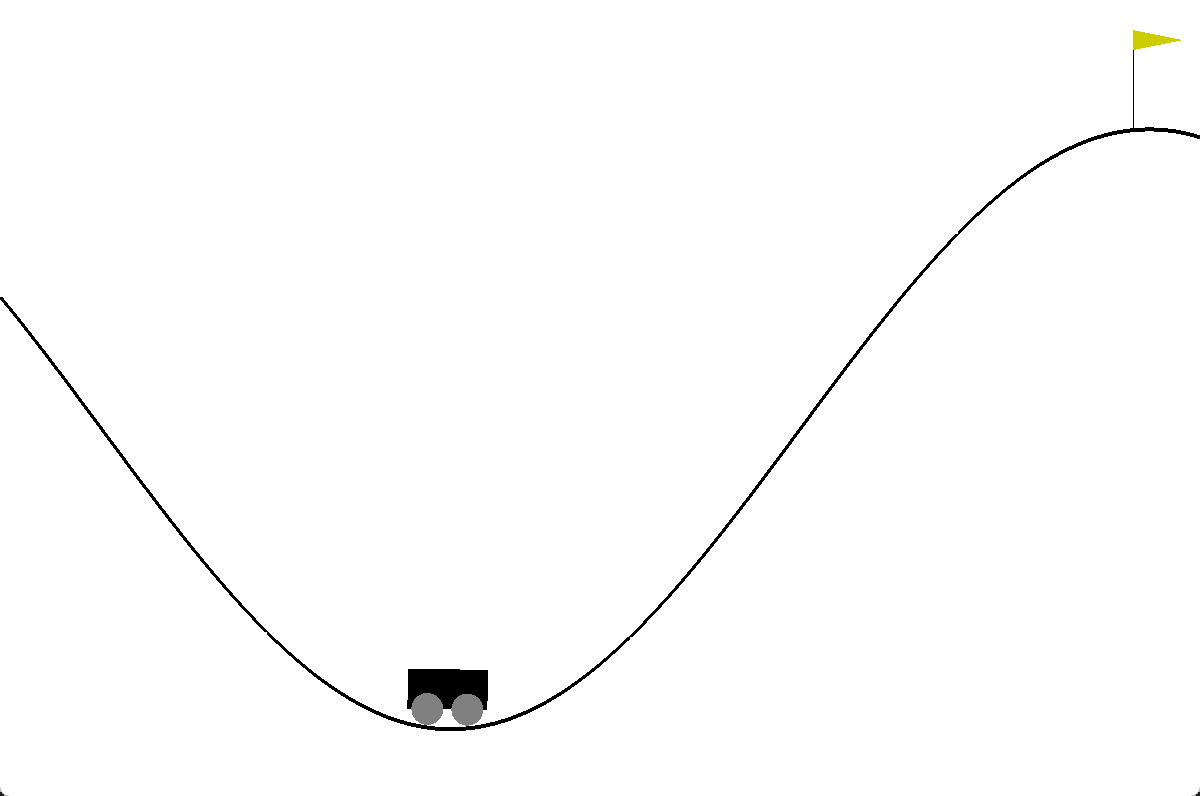
\includegraphics[width=0.5\linewidth]{figs/MountainCar.png}
    \caption{What the Mountain Car environment looks like. The car starts at some point in the valley. The goal is to get to the top right flag.}
    \label{fig:mountaincar}
\end{figure}

The state of the environment is represented by two variables, \texttt{position} and \texttt{velocity}. \texttt{position} can be between $-1.2$ and $0.6$ inclusive and \texttt{velocity} can be between $-0.07$ and $0.07$ inclusive. These are just measurements along the $x$-axis.

The actions that you may take at any state are $\{0, 1, 2\}$ which respectively correspond to (0) pushing the car left, (1) doing nothing, and (2) pushing the car right.

\subsection{Q-learning With Linear Approximations}
The Q-learning algorithm is a model-free reinforcement learning algorithm where we assume we don't have access to the model of the environment we're interacting with. We also don't build a complete model of the environment during the learning process. A learning agent interacts with the environment solely based on calls to \textbf{step} and \textbf{reset} methods of the environment. Then the Q-learning algorithm updates the q-values based on the values returned by these methods. Analogously, in the approximation setting the algorithm will instead update the parameters of q-value approximator.


Let the learning rate be $\alpha$ and discount factor be $\gamma$. Recall that we have the information after one interaction with the environment, $(s, a, r, s')$. The tabular update rule based on this information is: 
\[
    Q(s,a) = (1 - \alpha) Q(s, a) + \alpha \left(r + \gamma \max_{a'} Q(s', a')\right)
\]

Instead, for the function approximation setting we get the following update rule derived from Section~\ref{sec:FA}\footnote{Note that we have made the bias term explicit here, where before it was implicitly folded into $\wv$ }:

\[
\wv \leftarrow \wv - \alpha \left(q(\sv, a; \wv) - (r + \gamma \max_{a'} q(\sv', a'; \wv)\right) \nabla_\wv q(\sv, a; \wv)
\]

Where:

\[
q(\sv,a;\wv) = \sv^T \wv_a + b
\]

The epsilon-greedy action selection method selects the optimal action with probability $1 - \epsilon$ and selects uniformly at random from one of the 3 actions (0, 1, 2) with probability $\epsilon$. The reason that we use an epsilon-greedy action selection is we would like the agent to do explorations as well. For the purpose of testing, we will test two cases: $\epsilon = 0$ and $0 < \epsilon < 1$. When $\epsilon = 0$, the program becomes deterministic and your output have to match our reference output accurately. In this case, if there is a draw in the greedy action selection process, pick the action represented by the smallest number. For example, if we're at state $s$ and $Q(s, 0) = Q(s, 2)$, then take action $0$. And when $0 < \epsilon < 1$, your reference output will need to fall in a certain range that we determine by running exhaustive experiments based on the input parameters.


\subsection{Feature Engineering}
Linear approximations are great in their ease of use and implementations. However, there sometimes is a downside; they're \emph{linear}. This can pose a problem when we think the value function itself is nonlinear with respect to the state. For example, we may want the value function to be symmetric about 0 velocity. To combat this issue we could throw a more complex approximator at this problem, like a neural network. But we want to maintain simplicity in this assignment, so instead we will look at a nonlinear transformation of the ``raw'' state.

\begin{figure}[H]
\centering
\begin{subfigure}{0.5\textwidth}

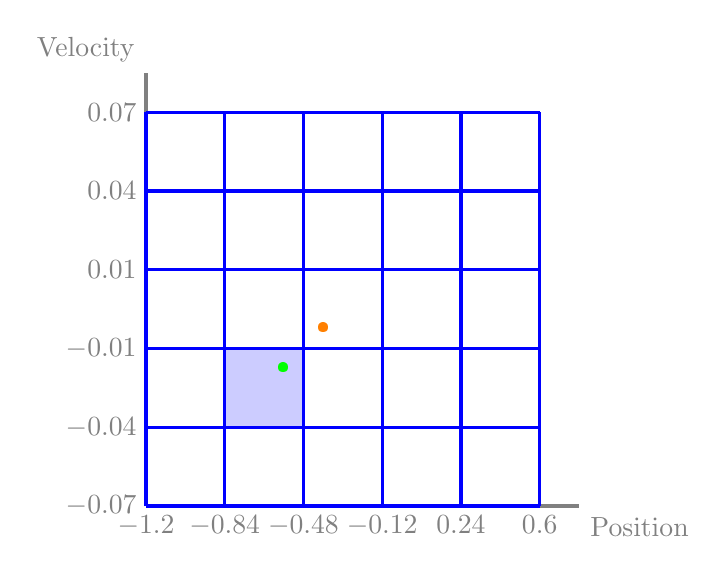
\begin{tikzpicture}[scale=1.0]
% https://tex.stackexchange.com/questions/45808/tikz-grid-lines
% https://tex.stackexchange.com/questions/305138/modify-the-scale-of-x-axis-and-y-axis
\pgfkeys{/pgf/number format/.cd,fixed,precision=2}
% Draw labels
\draw [ultra thick,gray,] (0,0)--(5.5,0) node[below right] {\text{Position}};
\draw [ultra thick,gray,] (0,0)--(0,5.5) node[above left] {\text{Velocity}};
% Draw axis
\newcommand*{\xMin}{0}%
\newcommand*{\xMax}{5}%
\newcommand*{\yMin}{0}%
\newcommand*{\yMax}{5}%
    \foreach \i in {\xMin,...,\xMax} {
        \draw [very thin,gray] (\i,\yMin) -- (\i,\yMax)  node [below] at (\i,\yMin) {\pgfmathparse{(\i/50)*18-1.2}$\pgfmathprintnumber{\pgfmathresult}$};
    }
    \foreach \i in {\yMin,...,\yMax} {
        \draw [very thin,gray] (\xMin,\i) -- (\xMax,\i) node [left] at (\xMin,\i) {\pgfmathparse{(\i/500)*14-0.07}$\pgfmathprintnumber{\pgfmathresult}$};
    }
% Draw grids
\draw [step=1.0,blue, very thick] (0.0,0.0) grid (5.0,5.0);
% \draw [very thick, red, step=1.0cm,xshift=-0.5cm, yshift=-0.5cm] (0.5,0.5) grid +(5.0,5.0);

% Draw shaded regions
\fill [blue, opacity=0.2] (1,1) rectangle (2,2);
% \fill [red, opacity=0.2] (1.5,1.5) rectangle (2.5,2.5);

% Draw point
\node [green] at (1.75,1.75) {\textbullet};
\node [orange] at (2.25, 2.25) {\textbullet};

\end{tikzpicture}
\caption{A discretization of the state space of Mountain Car}
\label{fig:discrete}
\end{subfigure}%
\begin{subfigure}{0.5\textwidth}

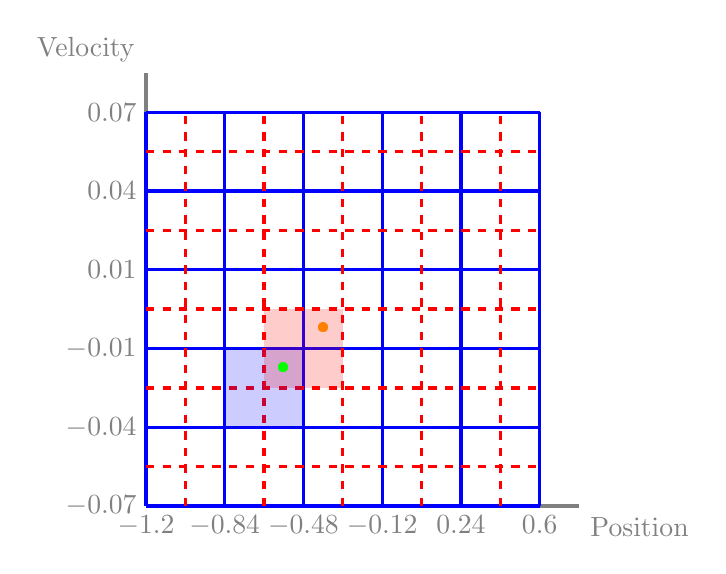
\begin{tikzpicture}[scale=1.0]
% https://tex.stackexchange.com/questions/45808/tikz-grid-lines
% https://tex.stackexchange.com/questions/305138/modify-the-scale-of-x-axis-and-y-axis
\pgfkeys{/pgf/number format/.cd,fixed,precision=2}
% Draw labels
\draw [ultra thick,gray,] (0,0)--(5.5,0) node[below right] {\text{Position}};
\draw [ultra thick,gray,] (0,0)--(0,5.5) node[above left] {\text{Velocity}};
% Draw axis
\newcommand*{\xMin}{0}%
\newcommand*{\xMax}{5}%
\newcommand*{\yMin}{0}%
\newcommand*{\yMax}{5}%
    \foreach \i in {\xMin,...,\xMax} {
        \draw [very thin,gray] (\i,\yMin) -- (\i,\yMax)  node [below] at (\i,\yMin) {\pgfmathparse{(\i/50)*18-1.2}$\pgfmathprintnumber{\pgfmathresult}$};
    }
    \foreach \i in {\yMin,...,\yMax} {
        \draw [very thin,gray] (\xMin,\i) -- (\xMax,\i) node [left] at (\xMin,\i) {\pgfmathparse{(\i/500)*14-0.07}$\pgfmathprintnumber{\pgfmathresult}$};
    }
% Draw grids
\draw [step=1.0,blue, very thick] (0.0,0.0) grid (5.0,5.0);
\draw [very thick, dashed, red, step=1.0cm,xshift=-0.5cm, yshift=-0.5cm] (0.5,0.5) grid +(5.0,5.0);

% Draw shaded regions
\fill [blue, opacity=0.2] (1,1) rectangle (2,2);
\fill [red, opacity=0.2] (1.5,1.5) rectangle (2.5,2.5);

% Draw point
\node [green] at (1.75,1.75) {\textbullet};
\node [orange] at (2.25, 2.25) {\textbullet};

\end{tikzpicture}
\caption{A tiling of the state space of Mountain Car}
\label{fig:tiling}
\end{subfigure}

\caption{State representations for the states of Mountain Car}
\label{fig:states}
\end{figure}

For the Mountain Car environment, we know that \texttt{position} and \texttt{velocity} are both bounded. What we can do is draw a grid over the possible \texttt{position}-\texttt{velocity} combinations as seen in Figure~\ref{fig:discrete}. We then enumerate the grid from bottom left to top right, row by row. Then we map all states that fall into a grid square with the corresponding one-hot encoding of the grid number. For efficiency reasons we will just use the index that is non-zero. For example the green point would be mapped to $\{6\}$. This is called a \emph{discretization} of the state space.

The downside to the above approach is that although observing the green point will let us learn parameters that generalize to other points in the shaded blue region, we will not be able to generalize to the orange point even though it is nearby. We can instead draw two grids over the state space, each offset slightly from each other as in Figure~\ref{fig:tiling}. Now we can map the green point to two indices, one for each grid, and get $\{6, 39\}$. Now the green point has parameters that generalize to points that map to $\{6\}$ (the blue shaded region) in the first discretization and parameters that generalize to points that map to $\{39\}$ (the red shaded region) in the second. We can generalize this to multiple grids, which is what we do in practice. This is called a \emph{tiling} or a \emph{coarse-coding} of the state space. 


\subsection{Implementation Details}
Here we describe the API to interact with the Mountain Car environment available to you in Python. The other languages will have an analagous API.

\begin{itemize}
    \item \texttt{\_\_init\_\_(mode)}: Initializes the environment to the a mode specified by the value of \texttt{mode}. This can be a string of either ``raw'' or ``tile''. 
    
    ``raw'' mode tells the environment to give you the state representation of raw features encoded in a sparse format: $\{0 \rightarrow \texttt{position}, 1 \rightarrow \texttt{velocity}\}$.
    
    In ``tile'' mode you are given indices of the tiles which are active in a sparse format: $\{T_1 \rightarrow 1, T_2 \rightarrow 1, \ldots T_n \rightarrow 1\}$ where $T_i$ is the tile index for the $i$th tiling. All other tile indices are assumed to map to 0. For example the state representation of the example in Figure~\ref{fig:tiling} would become $\{6 \rightarrow 1, 39 \rightarrow 1\}$.
    
    The size of the state space of the ``raw'' mode is 2. The size of the state space of the ``tile'' mode is 2048. These values can be accessed from the environment through the \texttt{state\_space} property, and similarly for other languages.
    \item \texttt{reset()}: Reset the environment to starting conditions.
    \item \texttt{step(action)}: Take a step in the environment with the given action. \texttt{action} must be either $0$, $1$ or $2$. This will return a tuple of $(\texttt{state}, \texttt{reward}, \texttt{done})$ which is the next state, the reward observed, and a boolean indicating if you reached the goal or not, ending the episode. The \texttt{state} will be either a raw' or tile representation, as defined above, depending on how you initialized Mountain Car.  If you observe \texttt{done = True} then you should \texttt{reset} the environment and end the episode. Failure to do so will result in undefined behavior.
    \item \textbf{[Python Only]} \texttt{render(self)}: Optionally render the environment. It is computationally intensive to render graphics, so only render a full episode once every 100 or 1000 episodes. Requires the installation of \texttt{pyglet}. This will be a no-op in autolab.
\end{itemize}

You should now implement your Q-learning algorithm with linear approximations as \newline\texttt{q\_learning.\{py|java|cpp|m\}}. The program will assume access to a given environment file(s) which contains the Mountain Car environment which we have given you. Initialize the parameters of the linear model with all 0 (and don't forget to include a bias!) and use the epsilon-greedy strategy for action selection.

Your program should write a output file containing the total rewards (the returns) for every episode after running Q-learning algorithm. There should be one return per line.

Your program should also write an output file containing the weights of the linear model. The first line should be the value of the bias. Then the following $|\mathcal{S}| \times |\mathcal{A}|$ lines should be the values of weights, outputted in row major order\footnote{\url{https://en.wikipedia.org/wiki/Row-_and_column-major_order}}, assuming your weights are stored in a $|\mathcal{S}| \times |\mathcal{A}|$ matrix.

The autograder will use the following commands to call your function:

\begin{tabbing}
For Python: \=\texttt{\$ \textbf{python} q\_learning.\textbf{py} [args\dots]}\\
For Java: \>\texttt{\$ \textbf{javac} -cp "./lib/ejml-v0.33-libs/*:./" q\_learning.\textbf{java}};\\ \>  \texttt{\textbf{java} -cp "./lib/ejml-v0.33-libs/*:./" q\_learning [args\dots]}\\
For C++: \>\texttt{\$ \textbf{g++} -g -std=c++11 -I./lib q\_learning.\textbf{cpp}; ./a.out [args\dots]}\\
% For Octave: \>\texttt{\$ \textbf{octave} -qH q\_learning.\textbf{m} [args\dots]}
\end{tabbing}

Where above \texttt{[args\dots]} is a placeholder for command-line arguments: \texttt{<mode>} \texttt{<weight\_out>} \texttt{<returns\_out>} \texttt{<episodes>} \texttt{<max\_iterations>} \texttt{<epsilon>} \texttt{<gamma>} \texttt{<learning\_rate>}. These arguments are described in detail below:
\begin{enumerate}
    \item \texttt{<mode>}: mode to run the environment in. Should be either \texttt{``raw''} or \texttt{``tile''}.
    \item \texttt{<weight\_out>}: path to output the weights of the linear model.
    \item \texttt{<returns\_out>}: path to output the returns of the agent
    \item \texttt{<episodes>}: the number of episodes your program should train the agent for. One episode is a sequence of states, actions and rewards, which ends with terminal state or ends when the maximum episode length has been reached.
    \item \texttt{<max\_iterations>}: the maximum of the length of an episode. When this is reached, we terminate the current episode.
    \item \texttt{<epsilon>}: the value $\epsilon$ for the epsilon-greedy strategy
    \item \texttt{<gamma>}: the discount factor $\gamma$.
    \item \texttt{<learning\_rate>}: the learning rate $\alpha$ of the Q-learning algorithm
\end{enumerate}


Example command for python users:
\begin{lstlisting}[language=Shell]
$ python q_learning.py raw weight.out returns.out \ 
 4 200 0.05 0.99 0.01
\end{lstlisting}

Example output from running the above command (your code won't match exactly, but should be close).

\texttt{<weight\_out>}
\begin{lstlisting}
-7.6610506220312296
1.3440159024460183
1.344872959883069
1.340055578403996
-0.0007770480987990149
0.0011306483117300896
0.0017559989206646666
\end{lstlisting}

\texttt{<returns\_out>}
\begin{lstlisting}
-200.0
-200.0
-200.0
-200.0
\end{lstlisting}

\subsection{Autolab Submission}
You must submit a .tar file 
named \texttt{rl.tar} containing \texttt{q\_learning.\{py|m|java|cpp\}}.  

You can create that file by running:
\begin{lstlisting}
tar -cvf rl.tar q_learning.{py|m|java|cpp}
\end{lstlisting}
from the directory containing your code. You may make up to \textbf{10 submissions} to Autolab before the deadline, but only your last submission will be graded.

Some additional tips: {\bf DO NOT} compress your files; you are just
creating a tarball. Do not use tar \texttt{-czvf}.  {\bf DO NOT} put
the above files in a folder and then tar the folder.  Autolab is case
sensitive, so observe that all your files should be named in {\bf
  lowercase}. You must submit this file to the corresponding homework
link on Autolab. The autograder for Autolab prints out some additional 
information about the tests that it ran. You can view this output by selecting 
 "Handin History" from the menu and then clicking one of the scores you 
 received for a submission. For example on this assignment, among other things, 
 the autograder will print out which language it detects (e.g. Python, Octave, C++, Java). 
 
 \begin{notebox}
  {\bf Python3 Users:} Please include a blank file called python3.txt (case-sensitive) in your tar submission and we will execute your submitted program using Python 3 instead of Python 2.7. Please do not rely on any ordering of dictionary elements.
 \end{notebox}

%\clearpage

\begin{notebox}
\paragraph{Linear Algebra Libraries} It is often more convenient to have a linear algebra library at your disposal. In this assignment, Java users may use EJML\footnote{\url{https://ejml.org}} and C++ users Eigen\footnote{\url{http://eigen.tuxfamily.org/}}. Details below. 
%
(As usual, Python users have numpy; Octave users have built-in matrix support.)
%
\begin{description}
\item[Java] EJML is a pure Java linear algebra package with three interfaces. We strongly recommend using the SimpleMatrix interface. Autolab will use EJML version 3.3. The command line arguments above demonstrate how we will call you code. The classpath inclusion \lstinline{-cp "./lib/ejml-v0.33-libs/*:./"} will ensure that all the EJML jars are on the classpath as well as your code. 
\item[C++] Eigen is a header-only library, so there is no linking to worry about---just \lstinline{#include} whatever components you need. Autolab will use Eigen version 3.3.4. The command line arguments above demonstrate how we will call you code. The argument \lstinline{-I./lib} will include the \lstinline{lib/Eigen} subdirectory, which contains all the headers.
\end{description} 
We have included the correct versions of EJML/Eigen in the handout.tar for your convenience. Do {\bf not} include EJML or Eigen in your Autolab submission tar; the autograder will ensure that they are in place. 
\end{notebox}